\documentclass{beamer}


\usepackage{todonotes}
\usepackage{ragged2e}
\usepackage[none]{hyphenat}

\usetheme{default}
\usecolortheme{beaver}



\setbeamerfont{page number in head/foot}{size=\large}
\setbeamertemplate{footline}[frame number]
\addtobeamertemplate{block begin}{}{\justifying}

\title{Investment Value of Education in the U.S. and Europe}

\author{  
\texorpdfstring{
\begin{table}[]
\centering
\begin{tabular}{l|r}
Nathaniel Bechhofer $\star$ & \url{nbechhof@gmu.edu} \\
Omnia Elemary & \url{oelemary@gmu.edu} \\
Iman Khalil & \url{ikhalil2@gmu.edu} \\
Jaclyn Lasky & \url{jlasky2@gmu.edu} \\
Yuran (Helena) Niu & \url{yniu3@gmu.edu} \\
\end{tabular}
\end{table}
Team 4
}{People}
}

\date{\today}

\let\olditem=\item
\renewcommand{\item}{\olditem \justifying}

\begin{document}
\justify

\frame{\titlepage} % Slide 1 (title, team members, emails, team leader) 



\frame % Slide 2 Problem : Relation to Data Mining and Application/Utility; Challenges; Background
{
  \frametitle{How does education predict income?}
 \begin{block}{Problem}
  We'd like to find out how much we can infer about someone's income from their education, 
  both in the United States and Europe. 
  \end{block}
  
  \begin{block}{Why it matters}
  If income matters for variables of interest from health to happiness, we can make indirect inferences about individuals and groups using individual or average education levels \textit{combined with other information}. 
  \end{block}
  
  \begin{small}
  \begin{block}{Some motivating facts}
  \begin{itemize}
  \item \href{https://www.clevelandfed.org/newsroom-and-events/publications/economic-commentary/2012-economic-commentaries/ec-201210-the-college-wage-premium.aspx}{``College degree holders enjoy an 84 percent increase in earnings over their high-school-educated counterparts [in the United States].''} 
  \item \href{http://inequality.org/oecd-report-inequality-rising-faster/}{In the United States, income earners at the 90th percentile make roughly 16 times as much as those at the 10th percentile.}
  \item \href{http://csweb.brookings.edu/content/research/essays/2014/saving-horatio-alger.html}{Americans born in the bottom income quintile have a 10\% chance of entering the top quintile. That probability \textbf{doubles} with a college degree.}
  \end{itemize}
  \end{block}
\end{small}

}

\frame % Slide 3 
{
  \frametitle{Data Sources}
  We use two datasets:
  \begin{itemize} 
  \item \href{http://www.europeansocialsurvey.org/}{European Social Survey (ESS)} 
  \item \href{https://cps.ipums.org/cps/index.shtml}{United States Current Population Survey (CPS)}
  \end{itemize}
  We obtained data files from the ESS website and the IPUMS (Integrated Public Use Microdata Series) in \texttt{dta} and \texttt{dat} formats.
  \begin{itemize}
  \item Both datasets are from the years 2010, 2012, and 2014.
  \item Both datasets contain rich information about respondents.
  \item We can use the US data from 2011, 2013, and 2015 to test (some of) our predictions.
  \end{itemize}
  The US data has 610,756 observations; the ESS data has 157,261 observations.
}

\frame % Slide 4
{
  \frametitle{Features}
Our dependent variable is measured differently in these datasets: the ESS gives us within country deciles, while the CPS gives a numerical answer in dollars.

For both data sets, we have variables telling us the following about respondents:
  \begin{itemize}
  \item Educational Attainment
  \item Age
  \item Gender
  \end{itemize}
  
  The Annual Social and Economic Supplement (ASEC) data from the CPS (obtained every March) that we are using has rich data about the occupation and employment status of respondents, which can help us clarify how education affects income.

}




\frame % Slide 5 Architecture
{
  \frametitle{Architecture}
  \begin{itemize}
  \item For the ESS, we obtained a \texttt{dta} file with missing values and value labels already applied.
  \item We used the software Stata to apply given data definitions from IPUMS to the CPS \texttt{dat} file to obtain an informative \texttt{dta} file.  
  \item With \texttt{pandas}, a Python package, we read the \texttt{dta} files as \texttt{DataFrame} objects to use in a Python 3.5 ecosystem.
  \item Within this ecosystem, we used the \texttt{matplotlib} and \texttt{seaborn} packages for exploratory visualization.
  \end{itemize}



  
}

\frame % Slide 6
{
  \frametitle{Preprocessing}

 For the US, we only analyze those between the ages of 30 and 34 making between \$10K and \$500K. 
 
 We recoded our categorial predictors as dummy variables: 
 \begin{itemize}
 \item Whether the person has a college degree (for education).
 \item If the person is female (for gender).
 \item If the person is looking for work or has found work (for labor force status).
 \end{itemize}
 
 Moreover, we use the natural log of income as our outcome variable, rather than income itself. Consequently, the fact that $\ln(1+x) \approx x$ means that differences in outcomes can be interpreted as percentage differences; i.e. predicting an increase of 0.1 in our outcome variable corresponds to an approximately 10\% increase in income.


}

\frame % Slide 7
{
  \frametitle{Normalization}


\begin{block}{Why use the natural log of income?}
  \begin{itemize}
  \item The distribution of the natural log of income is closer to a Gaussian. 
  \item Economists typically model earnings as a function of education and work experience using the \emph{Mincer equation}, which assumes complementarity.
  \end{itemize}
  \end{block}

\begin{figure}[htbp]
\begin{center}
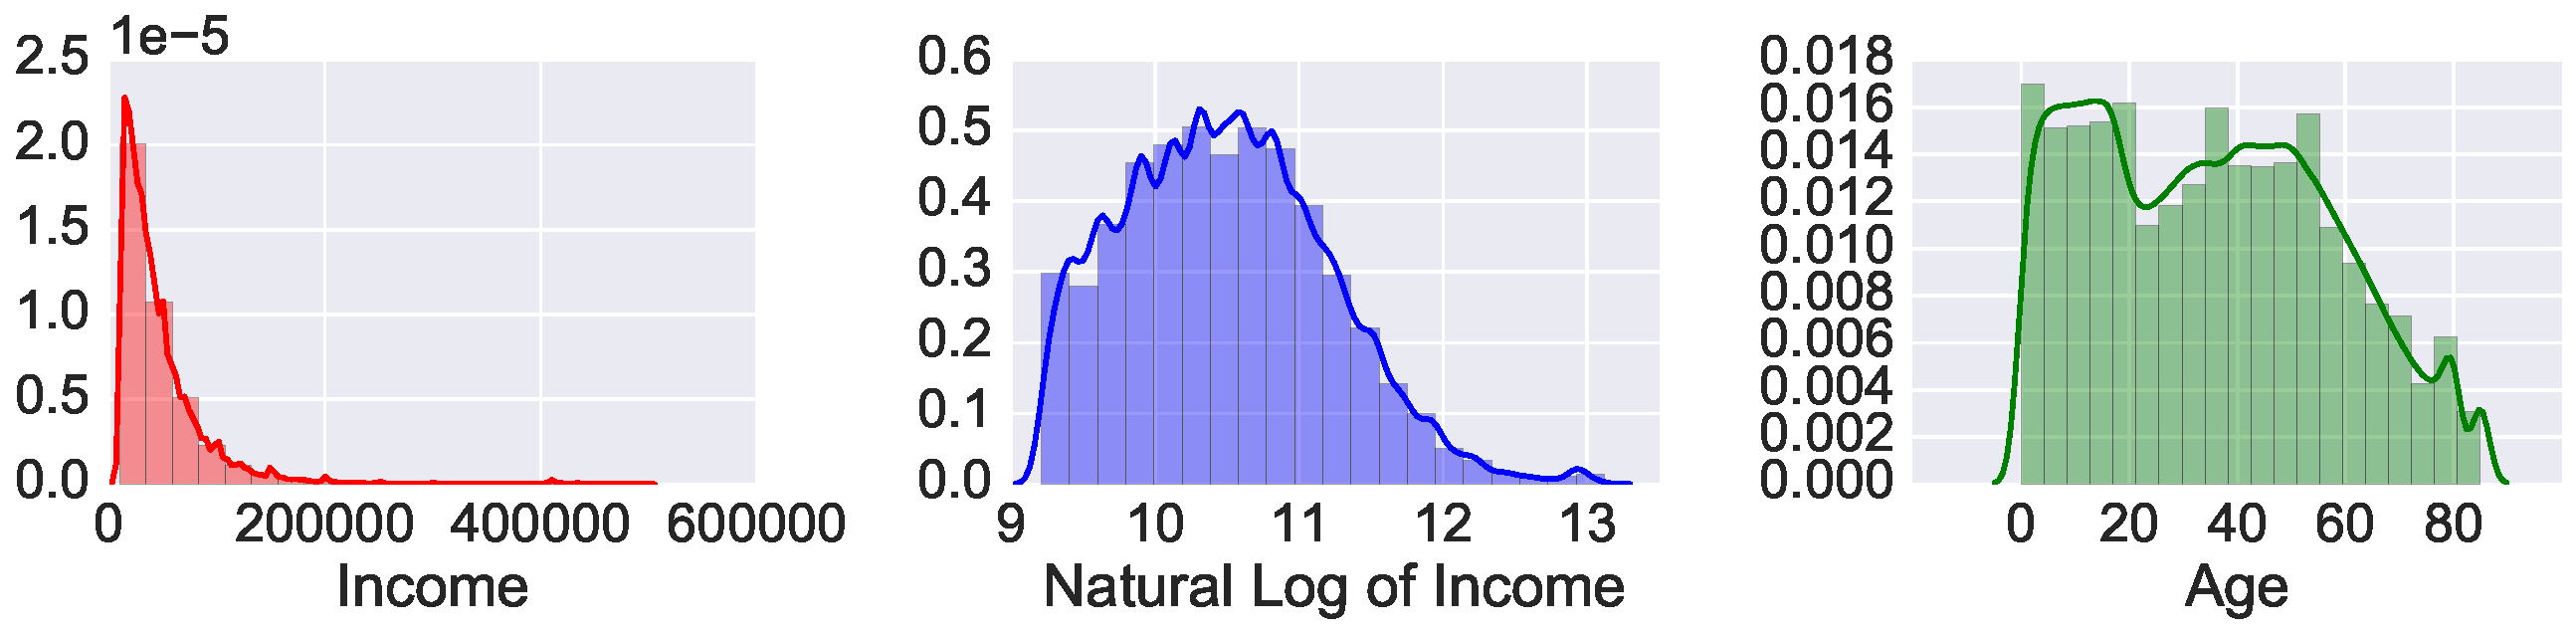
\includegraphics[width=\textwidth]{example_histograms.pdf}

\caption{Sample histograms from \texttt{seaborn}}
\label{histograms}
\end{center}
\end{figure}

}


\frame % Slide 8
{
  \frametitle{Feature Selection}
  To select features for prediction, we refer back to the basic problem: how can we best predict income using independent variables that have effects that are not operating via other independent variables include?
  
  We can expect that the effects of age or gender are not primarily operating via, e.g. education. 
  
  
  
}


\frame % Slide 9 Dimensionality Reduction
{
  \frametitle{Dimensionality Reduction}
  

Some variables we don't use:
\begin{itemize}
\item Whether one is currently in college
\item Birthplace 
\item Poverty 
\item Marital Status
\item Veteran Status
\end{itemize}

  We are currently working on reducing the dimensionality of occupation, to test whether the returns to education vary a lot by occupational choice.
 
  
  }
  

  

  



\frame % Slide 10 Model Selection
{
  \frametitle{Model Selection}
Our primary tool for model selection will be the $R^2$ values for linear regression. This calculates how much of the variation in measured income can be accounted for by the model. The values we obtain differ very little from those obtained when using an $R^2$ that penalizes for overfitting, as our sample size is large with every predictor both statistically and practically significant.
\vspace{48pt}


When working with the ESS data, which classifies income by deciles, we compute the total number of false positives, false negatives, and true positives over all classes, and then we compute precision, recall, and f-score using these counts. We then average these scores.   


  
  
  }
  
  \frame % Slide 11
  {
  \frametitle{Results from Linear Regression}
  \begin{Large}
  \begin{tabular}{l*{5}{c}}
\hline\hline
\hline
College   &       1.204&       1.201&       1.327&       1.324&       0.887\\
          &    (0.0337)&    (0.0337)&    (0.0328)&    (0.0328)&    (0.0277)\\
Age         &            &      0.0383&            &      0.0402&      0.0248\\
            &            &    (0.0114)&            &    (0.0110)&   (0.00924)\\
Female         &            &            &      -1.609&      -1.609&      -0.969\\
            &            &            &    (0.0312)&    (0.0312)&    (0.0267)\\
Worker     &            &            &            &            &       4.170\\
             &            &            &            &            &    (0.0318)\\
Constant       &       8.685&       7.461&       11.10&       9.817&       1.958\\
            &    (0.0198)&     (0.364)&    (0.0506)&     (0.355)&     (0.304)\\
\hline
\(N\)       &       41254&       41254&       41254&       41254&       41254\\
adj. \(R^{2}\)&       0.030&       0.030&       0.089&       0.089&       0.357\\
\hline\hline
\multicolumn{6}{l}{\footnotesize Standard errors in parentheses}\\
\end{tabular}

  \end{Large}

\vspace{12pt}

  For all of these regression results, our sample is all between the ages of 30 and 34 and with income between \$10000 and \$500000.
  
  }
  
  \frame % Slide 12
  {
  \frametitle{Evaluation}
  
  For all of our linear regression results, models with more predictors have increased $R^2$ values. 
  
  Moreover, we get consistent results for many of our coefficients, indicating relatively result estimation. 
  
  }

%\frame % Slide 13
%{
%  \frametitle{Ranked Performance}
%  
%  Right now, we have only used 
%  
%}

\frame % Slide 14
{
  \frametitle{ML Algorithms}
  
  For the Regression Tree of maximum depth 2, we obtain an average cross validation score of 0.200 when using 4-fold cross validation. This increases to 0.222 when allowing the maximum depth to be 5, indicating that higher depth is unambiguously better for our purposes.
  
  To come (with the ESS categorical income categorization, where our problem turns into classification):
  \begin{itemize}
\item Classification Decision Trees
\item Back-propogation
\item Random Forests
\item AdaBoost
\end{itemize}

  
  
  
}

%\frame % Slide 15
%{
%  \frametitle{Details}
%  
%}
  
  
  
\frame % Slide 16 
{
  \frametitle{Prediction}
  
  We are currently in the process of importing the sequestered data for the CPS to test the predictions we made, along with testing for the effects within our dataset for people aged 35-39.
  
}

%\frame % Slide 17 
%{
%  \frametitle{Plots}
%  
%}



\frame % Slide 18 Platforms (of your choice) Software and Hardware
{
  \frametitle{Platforms}
  \begin{itemize}
  \item Python 3.5
  \item \texttt{pandas} dataframe (built on \texttt{NumPy})
  \item \texttt{sci-kit learn} for ML algorithms
  \item All brought together with the Jupyter Notebook
  \item Version control using Github
  \end{itemize}
}

\frame % Slide 19 Discussion
{
  \frametitle{Discussion}
  
  All of the variables included appear to be both statistically and practically significant; we plan to add in additional features that are available to us from both datasets.

}

\frame % Slide 20 Conclusions
{
  \frametitle{Conclusion}
  Education matters a lot for income. We get a remarkably good fit when using our log-linear model, indicating that education primarily affects how income changes, rather than income levels themselves. Further work might explore the interaction of education and age, along with hierarchical modeling that can incorporate variables than we excluded.

}



\end{document}
